\documentclass[10pt]{article}
\usepackage[margin=0.7in]{geometry}
\usepackage{amsmath}
\usepackage{graphicx}
\usepackage{listings}
%\usepackage{pythonhighlight} % This is dank af
\usepackage{subcaption}
\usepackage{float}
\usepackage{url}
\usepackage{cite}
\usepackage[final]{pdfpages}

% DEFINE DAT NABLA COMMAND 4 EASY LIVIN
\newcommand{\grad}{\vec{\nabla}}

\title{ASEN 5051\\ {\Large Mini-Project 2}}
\author{Lucas Calvert and Duncan McGough}
\date{Due soon in 2018}

\begin{document}
\maketitle

\tableofcontents
\listoffigures
\newpage

\section{Introduction}
In this project, the dynamics of the interaction between two ideal vortex rings was examined.\\

In theory, a vortex ring is formed when the two ends of a finite length \textit{vortex filament} are connected to eachother. This connection forms a ring of radius \textit{R}, with a strength $\Gamma$. While these rings are infintesimally small and have no mass, they do induce a velocity at a distance, due to the circulation about the rings. This velocity can be characterized relatively simply by applying the Biot-Savart Law:

\[ u_{induced} = \frac{\Gamma}{4\pi}\int_{c} \frac{\hat e_{\omega} \times (\vec x - \vec x')}{|(\vec x - \vec x')|} dl \]

Where $\hat e_{\omega}$ is the direction about which the vorticity acts about, $\vec x$ is the point where the velocity id being induced, $\vec x'$ is the "current" point on the vortex ring that is being integrated around and \textit{c} is the curve corresponding to one vortex ring. If we wanted to make a more general code to examine the interaction of any arbitrary (closed) vortex filament loops, it would involve using this integral to detemine the effects at every point, from every point on a filament. Luckily, however, in this project a special symmetry may be exploited, simplifying the problem and drastically reducing the coputational time required to run a simulation.

The simplifying assumption used is as follows: since we know (by our setup) that both vortex rings are initially perfectly circular, we can expect that they will remain circular for all time. Just by noticing this simple fact, we can now determine the motion of an entire vortex ring by analyzing the velocity induced at a \textbf{single point} along it. The application of this idea will be discussed further in the following sections.

It should also be noted that, in order to simplify the computations, this integral was converted from cartesian to polar coordinates. Knowing that: \[dl = Rd\theta\] \[x = Rcos(\theta)\] \[y = Rsin(\theta)\] We can tranform the terms in the Biot-Savart integral as follws: \[\vec x = [  Rcos(\theta) , Rsin(\theta)  , h  ]^T\] \[\vec x' = [  Rcos(\theta ') , Rsin(\theta '')  , h' ]^T\] \[e_{\omega} = [ sin(\theta ') , -cos(\theta '  , 0 ]^T\]

Where h is the distance from the y-z plane of the center of the respective ring. After making out subtitutions in the Biot-Savart equation, we can numerically integrate the equation about one of the rings (from 0 - 2$\pi$ in this case) using a trapezoidal apporximation. The result is the velocity induced from one entire ring at a single specified point.\\

Now that we have a method for numerically solving the Biot-Savart law, we can start to solve for the motion of the vortex rings. To do this, we first exploit a major simplification - since both rings start as perfect, radially symmetric, circles, we can expect that they will remain this shape for all time. This is to say that the only changes that occur will be changes in the size of both rings, and their distances away from the y-z plane. Furthermore, this means that if we can solve for the motion of \textit{one discrete point} on a ring, we can assume the rest of the rings follows the same motion.\\

To solve for the dynamics of the full problem,  the induced velocity effects were broken up into four parts - ring 1 on itself, ring 2 on itself and each ring on the other. In the code for simulating the motion, these four calculations are made at each time step, then the position and size of each ring is updated. The radius of each ring, the distance between the two rings as well as the cartesian positions of each point on the rings are plotted after each time step, producing an animation (or "movie", if you will) of the ring interaction. These plot, as well as text outputs of useful information, can be used to analyze the motion of the rings and produce empirical formulas for important characteristics of the interactions. This application of the code will be discussed further in the rest of this report.

\section{Task 1}

For this section the project, the interaction between "two vortex rings of identical strength and a similar sense of rotation" were analyed. It is expected that the rings will exhibit a "leap-frogging" frogging behavior where they move across the domain, moving inside and outside of eachother, which is exactly what happened.\\
With a time step 0f 0.2s, 100 discrete points in each ring, an initial radius of 1m and an initial distance apart 1m, the simulation was run for 50s. The resulting radius vs. time and horizontal distance between rings vs. time output plots are shown below:

\begin{figure}[H]
   \centering
   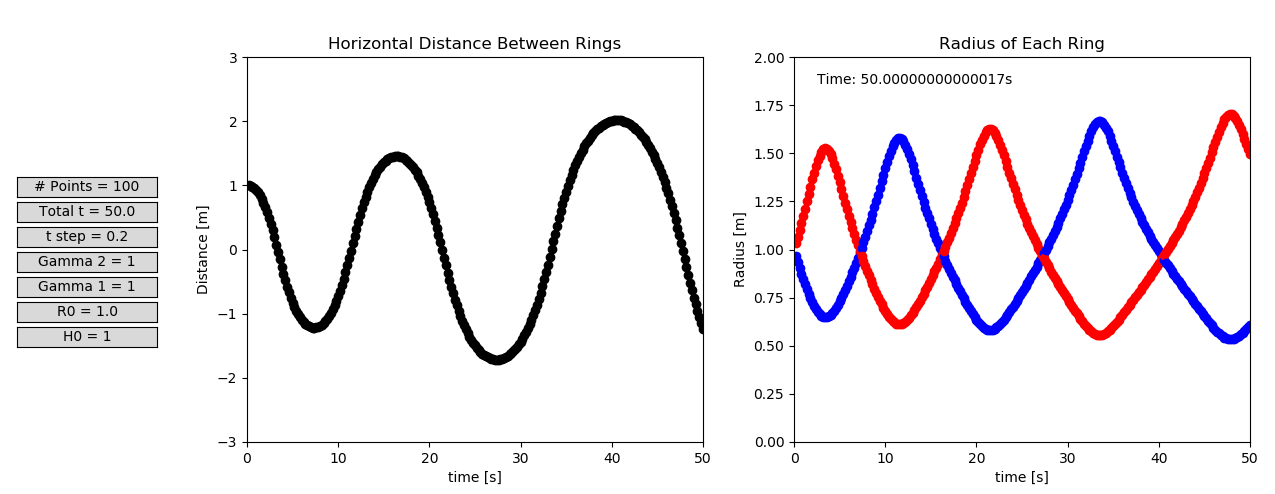
\includegraphics[width=1\linewidth]{figures/task1_coarse_lowD.png}
   \caption{Low Resolution, Low discretization Results}
   \label{task1_coarse_lowD}
\end{figure}


With these resolution settings (time step and discretization level), an unexpected behavior may be seen - that is: the rings begin to spread out and increase in maximum radius with every leapfrogging cycle. This is due to the nature of this numerical foreward-euler simulation. Errors in numerically evaluating the Biot-Savart integral complile, causing the simulation to diverge.\\

In an attempt to correct this behavior, the discretization level was increased by an order of magnitude (from 100 points along each ring to 1000). The results are as follows:


\begin{figure}[H]
   \centering
   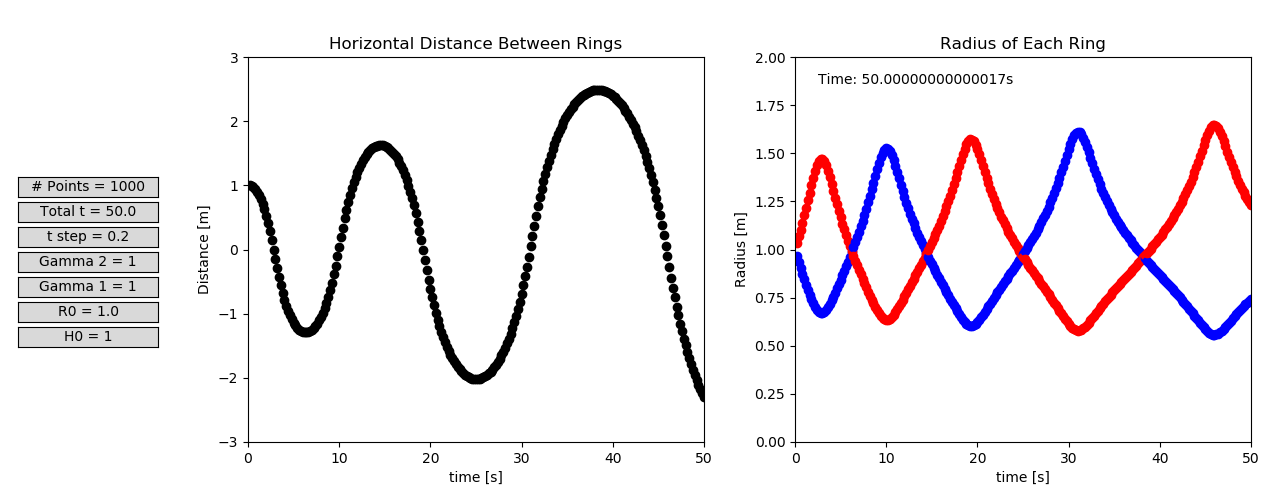
\includegraphics[width=1\linewidth]{figures/task1_coarse_highD.png}
   \caption{Low Resolution, High discretization Results}
   \label{task1_coarse_highD}
\end{figure}

Increasing the discretization level did not correct the result - it just made the simulation run for a longer time. Next, the time step was reduced drastically. Running the simulation again produced the following output:


\begin{figure}[H]
   \centering
   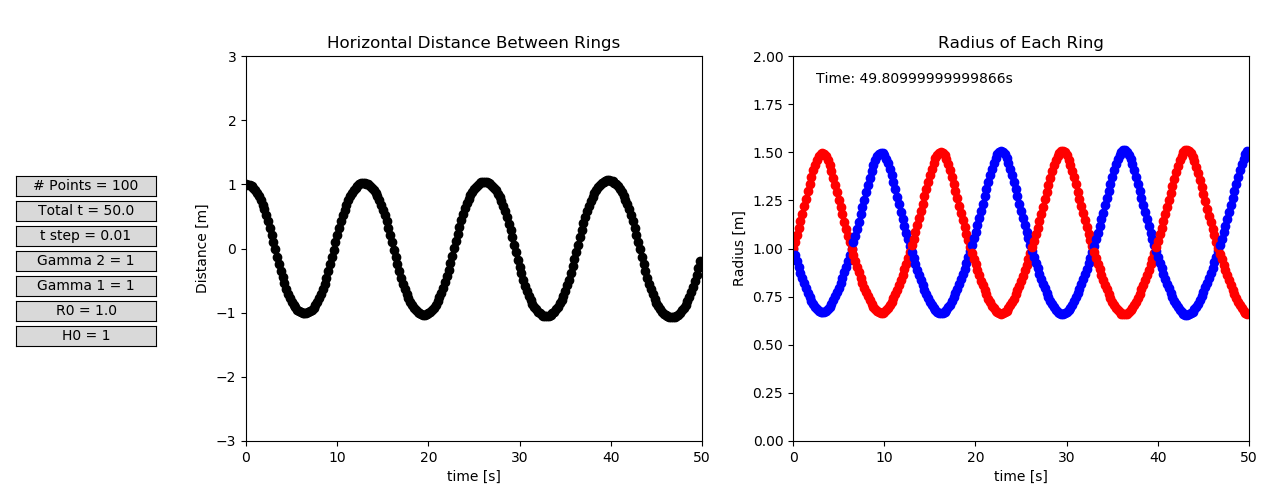
\includegraphics[width=1\linewidth]{figures/task1_fine.png}
   \caption{High Resolution (small time step) Results}
   \label{task1_fine}
\end{figure}


This adjustment (while it also caused the simulation to run noticeably slower) produced much better and consistent looking results. Figure \ref{task1_fine} shows a consistent period of "leap-frogging" and consistent radii for both rings.


Two videos (animations) of the transient states obsevred during this simulation are included with the submission of this report - one for the low resolution simulation with low discretization and on for the high resolution simulation. The videos are titled "task1\_lowRes.mp4" and "task1\_highRes.mp4", respectively.



\section{Task 2}

For this section of the project, the interaction between "two vortex rings of identical strength and an opposite sense of rotation" was examined. In much the same was as with the first task, the simulation was first run with ethe "low resolution" settings from before. The initial setup was such that the initial distance between the rings was 10m, their radii start at 1m, $\Gamma$ was set to 1 and the timestep was set to 0.2 seconds. The simulation was run for ****s to produce the following results:

\begin{figure}[H]
   \centering
   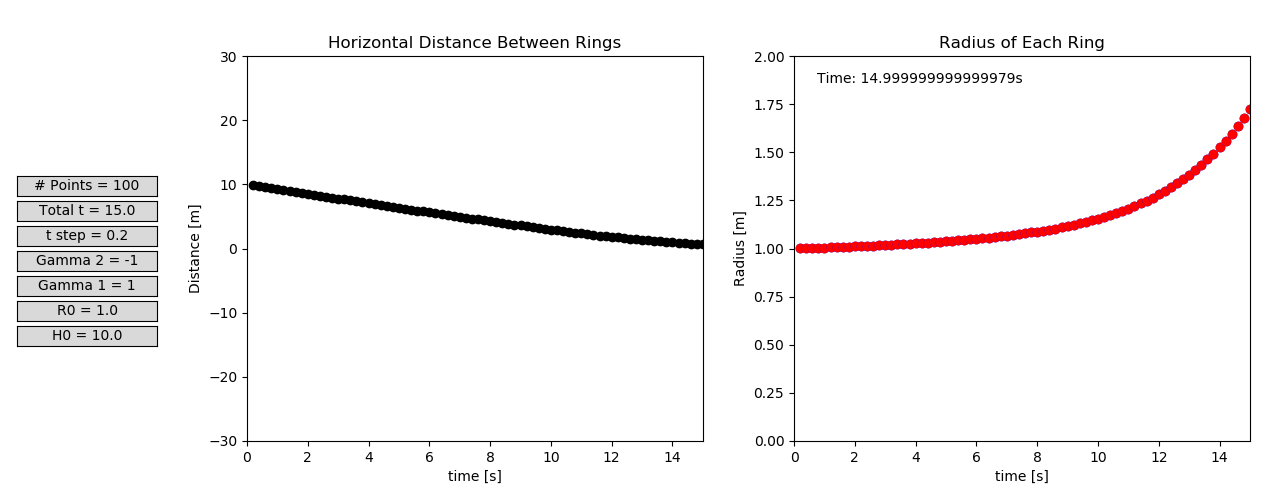
\includegraphics[width=1\linewidth]{figures/task2_coarse.png}
   \caption{Low Resolution Results}
   \label{task2_coarse}
\end{figure}


So that a comparison between fine and course time steps could also be made for this task, the time step value was again reduced to 0.01s. This produced the following results:


\begin{figure}[H]
   \centering
   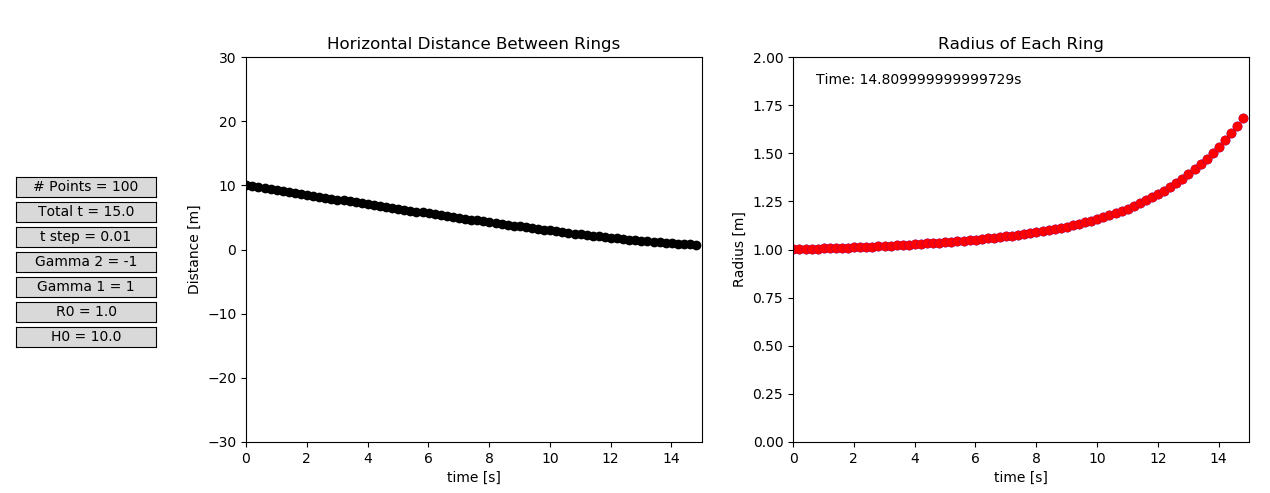
\includegraphics[width=1\linewidth]{figures/task2_fine.png}
   \caption{High Resolution Results}
   \label{task2_fine}
\end{figure}

In this case, refining the time step caused a much less noticeable change. This is likely due to the non-cyclic behavior of this setup. The results with the refined time step are likely more accurate, even if they are visually similar to the unrefined time step results.

Videos of both of these simulations have also been included with this submission.


\section{Task 3}
For this task, we want to determine an analytical formula for the time $T$ of a leapfrogging cycle in terms of $R,~H,$ and $\Gamma$. Let's start out by formulating the dimensional matrix:

\[\begin{matrix}
 & T & R & H & \Gamma \\ \hline
M & 0 & 0 & 0 & 0 \\
L & 0 & 1 & 1 & 2 \\
T & 1 & 0 & 0 & -1 \\
\end{matrix}\]

We can then take this matrix and use Gauss-Jordan to obtain the rank of the dimensional matrix:

\[\text{rref}\left(
\begin{bmatrix}
0 & 0 & 0 & 0 \\
0 & 1 & 1 & 2 \\
1 & 0 & 0 & -1 \\
\end{bmatrix} \right)
=
\begin{bmatrix}
1 & 0 & 0 & -1 \\
0 & 1 & 1 & 2 \\
0 & 0 & 0 & 0 \\
\end{bmatrix}
\rightarrow r=2
\]

Now, we determine the number of dimensionless groups $n-r$ where $n$ is the number of dimensional variables and $r$ is the rank of the dimensional matrix. $n-r=4-2=2$ dimensional groups.

Let:
\[\Pi_1=\frac{\Gamma T}{RH}\rightarrow\frac{L^2}{T}\frac{T}{1}\frac{1}{L}\frac{1}{L}\rightarrow \text{ dimensionless}\]

Let's choose our next Pi group:

\[\Pi_2=\frac{R}{H}\rightarrow \frac{L}{1}\frac{1}{L}\rightarrow \text{ dimensionless}\]

We can then formulate that:
\[\Pi_1=\psi(\Pi_2)\]
\[\frac{\Gamma T}{RH}=\psi\left(\frac{R}{H} \right)\]

We can select values for $\Gamma$, $R$, and $H$ and use the Python code developed in Tasks 1 and 2 to determine the complete leapfrog period $T$. This was done several times, and is tabulated in Table \ref{tab:data}.

\begin{table}[H]
    \centering
    \begin{tabular}{c c c c}
    $\Gamma$ [m$^2$/s]& $R$ [m]& $H$ [m]& $T$ [s] \\ \hline
    1 & 1 & 1 & 12.81 \\
    1 & 2 & 1 & 17.62 \\
    2 & 1 & 1 & 6.61 \\
    1.5 & 1.5 & 1 & 10.81 \\
    1 & 1 & 0.5 & 4.61 \\
    0.5 & 1 & 0.5 & 8.82 \\
    0.8 & 2 & 0.2 & 1.21 \\
    1 & 0.8 & 0.4 & 3.01 \\
    1.2 & 0.7 & 0.6 & 4.41 \\
    5 & 2 & 1 & 3.62 \\
    5 & 2 & 2 & 10.41 \\
    2 & 4 & 1 & 10.01 \\
    2 & 5 & 1 & 10.02 \\
    2 & 6 & 1 & 10.21 \\
    2 & 7 & 1 & 10.21 \\
    2.0 & 7 & 1.2 & 14.4 \\
    2 & 7.2 & 1.4 & 19.62 \\
    2 & 6.8 & 1.4 & 19.62 \\
    1.6 & 6.5 & 1.5 & 27.6 \\
    1 & 3 & 0.2 & 0.841 \\
    1 & 3 & 1 & 19.01 \\
    1 & 1.6 & 0.2 & 0.821 \\
    1 & 2.5 & 1 & 18.82 \\
    0.5 & 0.8 & 1 & 21.62 \\
    \end{tabular}
    \caption{Collected Data from Python Script for Complete Leapfrog}
    \label{tab:data}
\end{table}

Once the data is collected $\Pi_1$ is plotted versus $\Pi_2$. Then, an exponential curve can be fit to the data to obtain $\psi$. The plot and fitted curve can be seen in Figure \ref{fig:fit}.

\begin{figure}[H]
    \centering
    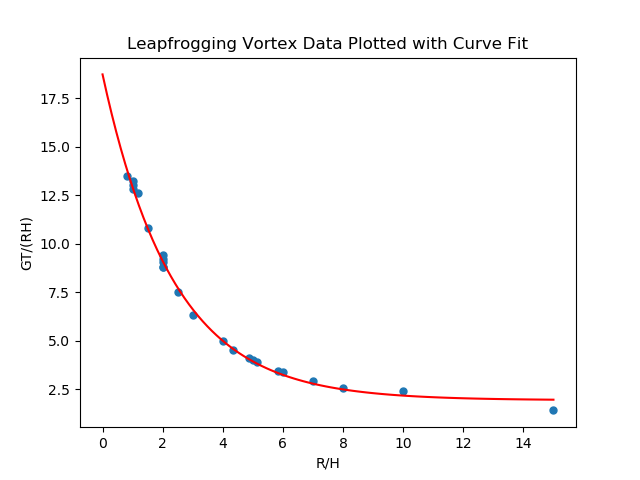
\includegraphics[width=0.7\linewidth]{figures/datafit.png}
    \caption{Collected Data Points for Leapfrogging Vortices}
    \label{fig:fit}
\end{figure}

This exponential curve takes the form:

\[\psi(x) = Ae^{-Bx} + C\]

The curve fitting in our Python script returns values of: $A=16.81$ and $B=0.425$ $C=1.926$.

The function can then be solved for $T$, leaving us with:

\[\boxed{T=\frac{RH}{\Gamma}\left[16.81e^{-0.425\frac{R}{H}}+1.926\right]}\]


To validate this empirical formula, the leap-frogging period for 3 test cases were calculated using both the formula and the Python code. The input parameters, results (from both methods) and percent error (considering the simulation as "truth") have been tabulated below:


\begin{table}[H]
    \centering
    \begin{tabular}{c c c c c c}
    $\Gamma$ [m$^2$/s]& $R$ [m]& $H$ [m]& $T_{simulation}$ [s] & $T_{formula}$ [s] & \% Difference \\ \hline
    1 & 1 & 1 & 12.81 & 12.92 & 0.86 \%\\
    1 & 2 & 0.5 & 5.02 & 5.000 & 0.40 \%\\
    3 & 3 & 1 & 6.61 & 6.62 & 0.15 \% \\
    \end{tabular}
    \caption{Collected Data from Python Script for Complete Leapfrog}
    \label{tab:error_analysis_1}
\end{table}

From table \ref{tab:error_analysis_1}, we can see the the formula derived above matched very closely to the values caluclated using the simulations, with an average error over the three test cases of $\mathbf{0.47\%}$

\section{Task 4}
Next we are interested when the vortex rings are separated by half their original distance, with their vortices having equal strength but opposite direction. The dimensional analysis used will be the same as in Task 3:

\[\frac{\Gamma T}{RH}=\psi\left(\frac{R}{H} \right)\]

Using our leapfrogging vortex Python script again, we can enter in data points and plot the results. The data points used are in Table \ref{tab:data2}.

\begin{table}[H]
    \centering
    \begin{tabular}{c c c c}
    $\Gamma$ [m$^2$/s]& $R$ [m]& $H$ [m]& $T$ [s] \\ \hline
    % G  R  H   T
    1 & 1 & 1 & 1.01 \\
    1 & 2 & 1 & 2.81 \\
    2 & 1 & 1 & 0.51 \\
    1.5 & 1.5 & 1 & 1.21 \\
    1 & 1 & 0.5 & 0.75 \\
    0.5 & 1 & 0.5 & 1.41 \\
    0.8 & 2 & 0.2 & 2.41 \\
    1 & 0.8 & 0.4 & 0.45\\
    1.2 & 0.7 & 0.6 & 0.405 \\
    5 & 2 & 1 & 0.561 \\
    5 & 2 & 2 & 0.841 \\
    2 & 4 & 1 & 4.4 \\
    2 & 5 & 1 & 7.01 \\
    2 & 6 & 1 & 10.4 \\
    2 & 7 & 1 & 14.3 \\
    2.0 & 7 & 1.2 & 13.8 \\
    2 & 7.2 & 1.4 &  13.8 \\
    2 & 6.8 & 1.4 &  12.7 \\
    1.6 & 6.5 & 1.5 & 14.3 \\
    1 & 3 & 1 & 5.4 \\
    1 & 1.6 & 0.2 & 1.21 \\
    1 & 2.5 & 1 & 4.0 \\
    0.5 & 0.8 & 1 & 1.61 \\
    \end{tabular}
    \caption{Collected Data from Python Script for Half Distance to Leapfrog}
    \label{tab:data2}
\end{table}


These data points were then input into another plotting and curve fitting Pyhton script. A linear fit was found for the data, and the results were plotted in figure \ref{fig:fit2} below.


\begin{figure}[H]
    \centering
    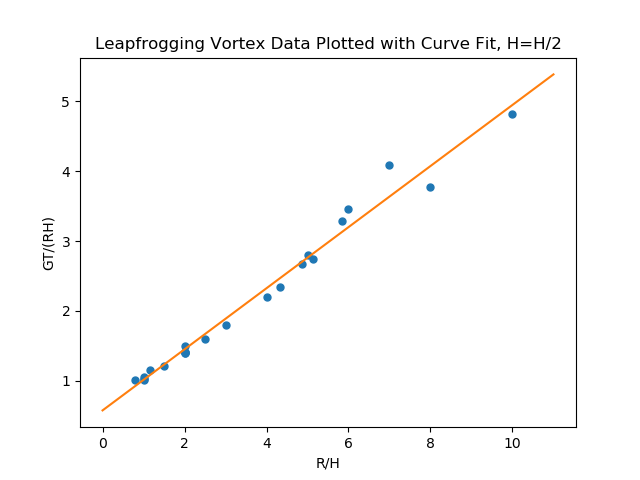
\includegraphics[width=0.7\linewidth]{figures/datafit_2.png}
    \caption{Collected Data for Expanding Vortices}
    \label{fig:fit2}
\end{figure}


From out fit line, we can see that:

\[\Pi1 = 0.437\Pi2 + 0.576  \]

Subsituting the parameters that make up the Pi groups and solving for T results in the following expression:

\[\boxed{T=\frac{RH}{\Gamma}(0.437(\frac{R}{H}) + 0.576)  ]}\]




To validate this empirical formula, the time the rings take to reach half of their starting separation distance for 3 test cases were calculated using both the formula and the Python code. The input parameters, results (from both methods) and percent error (considering the simulation as "truth") have been tabulated below:



\begin{table}[H]
    \centering
    \begin{tabular}{c c c c c c}
    $\Gamma$ [m$^2$/s]& $R$ [m]& $H$ [m]& $T_{simulation}$ [s] & $T_{formula}$ [s] & \% Difference \\ \hline
    1 & 1 & 10 & 6.91 & 6.197 & 10.3 \%\\
    2 & 4 & 6 & 11.05 & 10.41 & 5.8 \%\\
    6 & 1 & 6 & 0.71 & 0.65 &  8.4\% \\
    \end{tabular}
    \caption{Collected Data from Python Script for Complete Leapfrog}
    \label{tab:error_analysis_1}
\end{table}

From table \ref{tab:error_analysis_1}, we can see that the average error over the three test cases was $\mathbf{8.2\%}$. While this is not as low as the leap-frogging model, the error is still sufficiently low to validate the formula.

\section{Running the Code}

The simulation and plotting code for this project is fairly simple. First, make sure that you have Python 3 installed properly. Next, adjust the input parameters on lines 30-40 of "rings.py" (this is the script that performs the simulation). Save the file. To run, open a terminal window, navigate to the folder containing this submission on type "python rings.py" - the simulations should now run be visible on your screen. If the simulation runs slowly, try adjustinng the "tStep" and "displayValue" variables, as these will change the time step of the simulation and how often the plots are updated.

\end{document}
